% Licensed under the Creative Commons Attribution Share Alike 4.0 International.
% See the LICENSE file in the repository root for full license text.

\section{走近内存}

\subsection{物理存储器的抽象结构}

数字电路存储器大小的基本单位是\textbf{比特(bit)}。通俗地说,一个比特就是一位二进制数,就是一个开关。但\textbf{在计算机中,存储器的基本单元是字节(byte)},一个字节等于八个比特。我们可以把存储器看作格子,例如,下面是一个一比特的存储器,存有 $0$:
\begin{table}[H]
	\centering
	\begin{tabular}{|c|}
		\hline
		0
		\\\hline
	\end{tabular}
\end{table}

注意一比特的存储器要么存 $0$,要么存 $1$。同理,下面是一个八比特的存储器,存有二进制数\footnote{假设读者已经熟练掌握正整数的进制数转换。} $0100,0001_{(2)} = 65_{(10)}$:
\begin{table}[H]
	\centering
	\begin{tabular}{|c|c|c|c|c|c|c|c|}
		\hline
		0 & 1 & 0 & 0 & 0 & 0 & 0 & 1
		\\\hline
	\end{tabular}
\end{table}

由此可见,存储器存在“低位”和“高位”的概念。以上存储器的低位在右边,高位在左边,之后绘制这样的示意图时要注意标明哪边是低位或高位。由于计算机存储器的基本单元是字节,所以可以将以上八个比特合并为一个字节,示意图为:
\begin{table}[H]
	\centering
	\begin{tabular}{|c|}
		\hline
		$65_{(10)}$
		\\\hline
	\end{tabular}
\end{table}

不难发现,若把一个字节的存储器看作一个非负二进制整数,则其可以表示的范围是:
$$
0_{(10)} \sim 255_{(10)}
$$

现在我们只能用一个字节表示一个 $0$ 到 $255$ 的非负整数。之后的章节中我们将讨论如何使用数个字节\textbf{表示}不同类型的数据。

\subsection{虚拟内存}

我们常说“(物理)内存 $\SI{8}{G}$”,指的是我们的计算机中所有内存条(图 \ref{pic:ddr})的容量之和为 $\SI{8}{G}$ \textbf{字节}。在此语境下,$\si{G}$ 表示 $(10^3)^3 = 1000^3$ 或 $(2^{10})^3 = 1024^3$,商家一般会选择成本较低的那个含义。为了严谨,我们明确规定:$\SI{1}{GB}$ 表示 $(10^3)^3$ 字节,$\SI{1}{GiB}$ 表示 $(2^{10})^3$ 字节,其他类似单位同理。

\begin{figure}[ht]
	\centering
	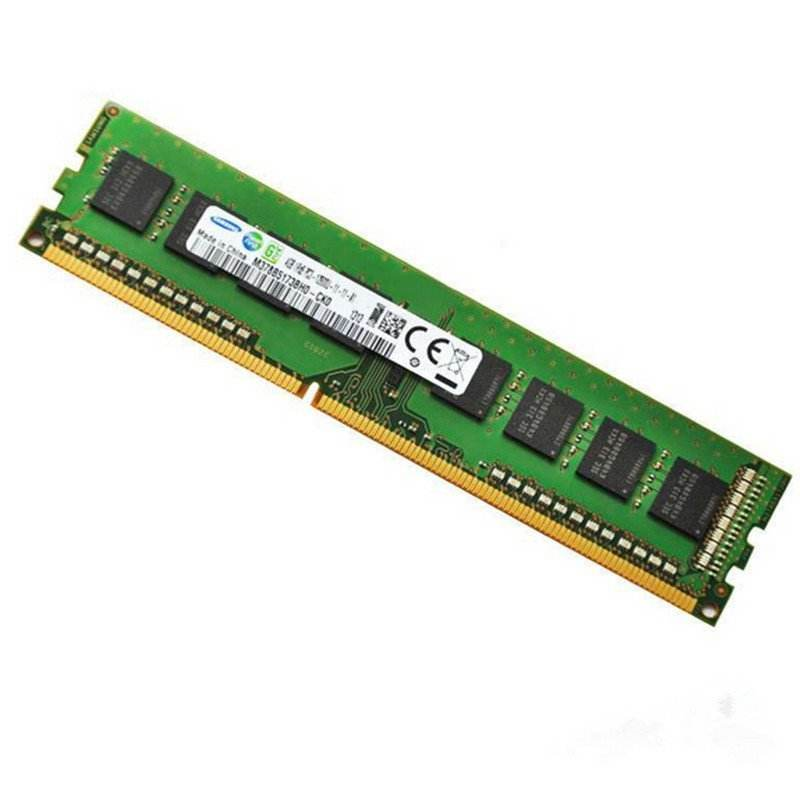
\includegraphics[width=0.5\linewidth]{pic/ddr.png}
	\caption{内存条}
	\label{pic:ddr}
\end{figure}

虽然我们的物理内存可能只有 $\SI{8}{GB}$,但在\textbf{操作系统与 CPU 硬件结构}的共同“保护”下,我们的程序并不直接读写物理内存。在逻辑上,这些程序读写的是\textbf{虚拟内存},看起来就像在\textbf{独享}一个非常大的\textbf{内存空间}。由于目前个人计算机的 CPU 均是 64 位的,所以对于个人计算机而言,虚拟内存空间的大小完全取决于操作系统的位数。32 位操作系统的虚拟空间大小为 $2^{32}$ 字节,等于 $\SI{4}{GiB}$;64 位操作系统的虚拟空间大小为 $2^{64}$ 字节,是 $\SI{4}{GiB}$ 的 $4294967296$ 倍\footnote{$2^{32} = 4294967296$}!

Windows 操作系统允许在 64 位系统中运行 32 位的程序,这些程序的虚拟空间大小仍然只有 $\SI{4}{GiB}$;较为先进的单片机往往是 32 位的,如果其中运行有操作系统,则操作系统中运行的程序的虚拟空间大小为 $\SI{4}{GiB}$。可见,“编写 32 位程序”与“编写 64 位程序”都是有需求的。使用高级语言编写通用的程序时,应当考虑“32 位”与“64 位”程序的区别。实践中,只有像 C/C++ 这样较为接近底层的语言需要考虑该事宜,更高级的语言无需理会这些区别。

\subsection{虚拟内存空间的极简结构}

以 64 位程序为例,前面提到,虚拟内存好似程序在独享一个非常大的空间,所以其基本结构为:
\begin{table}[H]
	\centering
	\begin{tabular}{|c|c|ccc|c|}
		\hline
		字节 $0$ & 字节 $1$ &  & $\cdots$ &  & 字节 $2^{64} - 1$
		\\\hline
	\end{tabular}
\end{table}

以上示意图表明,\textbf{可以将整个内存空间看作一列长表格}。程序读写内存时,最重要的特点是\textbf{随机读写},即可以根据\textbf{内存地址}找到该长表格中相应的存储单元,\textbf{在逻辑上,内存地址与查找速度没有关系}。例如,如果程序要读写从 $0$ 开始数的第 $114514$ 个内存单元,只需给出地址 $114514$,就能找到:
\begin{table}[H]
	\centering
	\begin{tabular}{|c|c|ccc|c|ccc|c|}
		\hline
		字节 $0$ & 字节 $1$ &  & $\cdots$ &  & 字节 $114514$ &  & $\cdots$ &  & 字节 $2^{64} - 1$
		\\\hline
	\end{tabular}
\end{table}

由于这是虚拟内存空间,所以称上例中的 $114514$ 为\textbf{虚拟地址}。受操作系统保护的程序保存的地址一定是虚拟地址,不会出现物理地址。虚拟地址到物理地址的转换由操作系统和 CPU 硬件结构完成,对一般的程序员是透明的。

程序可以随意读写虚拟地址吗?当然不行。程序只能在操作系统允许的虚拟地址范围内进行读写,不同区域的虚拟内存还具有不同的权限,有些区域只能读,很多区域不能被当作程序执行……幸运的是,如果编写的程序与虚拟内存无关\footnote{以修改内存为原理的游戏修改器显然与之有关,需要知道这些概念。},那么这些概念都是透明的。对于高级语言程序员来说,只要不写失格的代码,规范地向操作系统申请虚拟内存空间,就不会出问题。